\documentclass[12pt]{article}

\usepackage[top = 1in, bottom = 1in, left = 0.75in, right = 0.75in]{geometry}
\usepackage{amsmath, amssymb, amsthm}
\usepackage{graphicx}
\usepackage{float}
\usepackage{tikz}
\usetikzlibrary{shapes.geometric, arrows}

\tikzstyle{arrow} = [thick,->,>=stealth]
\tikzstyle{process} = [circle, minimum width=1.5cm, minimum height=1.5cm, text centered, draw=black]


\theoremstyle{definition}
\newtheorem{question}{Question}
\newenvironment{answer}{
    \textbf{\textit{Answer:}} \qquad
}{\hfill $\blacksquare$ \\ \begin{center}
    \rule{0.6\linewidth}{0.5px}    
\end{center}
}


% CUSTOM DEFINITIONS
\newcommand{\R}{\mathbb{R}}
\newcommand{\Z}{\mathbb{Z}}
\newcommand{\C}{\mathbb{C}}
\newcommand{\zcal}{\mathcal{Z}}
\newcommand{\inv}[1][1]{^{(- #1)}}


\title{Solution to Signal Processing Assignments I}
\author{Subhrajyoty Roy (MB1911)}
\date{\today}

\begin{document}
\maketitle

\begin{center}
    \rule{0.8\textwidth}{1px} 
\end{center}
\vspace*{2em}


% Q1
% DONE
\begin{question}
    Determine the magnitude and phase response of the multipath channel
    $$
    y(n) = x(n) + x(n - M)
    $$
    At what frequencies does $H(\omega) = 0$?
\end{question}

\begin{answer}
    Letting $X(\omega)$ and $Y(\omega)$ denote the DTFT of the signal $x(n)$ and $y(n)$ respectively, and taking DTFT on both sides of the above equation, we have 

    \begin{align*}
        & Y(\omega) = X(\omega) + e^{-j\omega M} X(\omega)\\
        \Rightarrow \qquad & Y(\omega) = X(\omega) (1 + e^{-j\omega M})\\
        \Rightarrow \qquad & H(\omega) = \dfrac{Y(\omega)}{X(\omega)} = e^{-j\omega (M/2)} (e^{j \omega (M/2)} + e^{-j\omega (M/2)})\\
        \Rightarrow \qquad & H(\omega) = 2e^{-j\omega (M/2)} \cos\left( \omega \dfrac{M}{2} \right)
    \end{align*}

    Clearly, $H(\omega) = 0$ if and only if $\cos(\omega (M/2)) = 0$, i.e. $\omega (M/2) = (2k+1)\dfrac{\pi}{2}$, for any $k \in \Z$. Thus, $\omega = \dfrac{(2k+1)\pi}{M}$, i.e. the frequencies when $H(\omega) = 0$ are $\pm \dfrac{\pi}{M}, \pm \dfrac{3\pi}{M}, \pm \dfrac{5\pi}{M}, \dots$.

\end{answer}


% Q2
% DONE
\begin{question}
    Determine the steady-state response of the system 
    $$
    y(n) = \dfrac{1}{2} [x(n) - x(n-2)]
    $$
    to the input signal 
    $$
    x(n) = 5 + 3\cos\left( \dfrac{\pi}{2}n + 60 \right) + 4 \sin(\pi n + 45) \qquad -\infty < n < \infty
    $$
\end{question}

\begin{answer}
    We start by computing the DTFT of both sides of the input output relationship given.

    \begin{align*}
        & Y(\omega) = \dfrac{1}{2} \left[ X(\omega) - e^{-2j\omega} X(\omega) \right]\\
        \Rightarrow \qquad & H(\omega) = \dfrac{Y(\omega)}{X(\omega)} = \dfrac{1}{2} (1 - e^{-2j\omega})
    \end{align*}

    We know that the input signal $x(n) = e^{j\theta n}$ is an eigenfunction to the LTI system with eigenvalue $\vert H(\theta) \vert$. Thus, we have the following:
    
    \begin{align*}
        \tau\left[1 \right] & = \dfrac{1}{2}(1 - 1) = 0\\
        \tau\left[e^{j(\pi/2)n} \right] & = \vert H(\pi/2) \vert e^{j(\pi/2)n} = \frac{1}{2}\vert (1 - e^{-j\pi}) \vert e^{j(\pi/2)n} = e^{j(\pi/2)n}\\
        \tau\left[e^{-j(\pi/2)n} \right] & = \vert H(-\pi/2) \vert e^{-j(\pi/2)n} = e^{-j(\pi/2)n}\\
        \tau\left[e^{j\pi n} \right] & = \vert H(\pi) \vert e^{j\pi n} = \frac{1}{2} \vert (1 - e^{-2j\pi}) \vert e^{j \pi n} = 0 \\
        \tau\left[e^{-j \pi n} \right] & = \vert H(-\pi) \vert e^{-j\pi n} = 0\\
    \end{align*}

    Hence,

    \begin{align*}
        \tau[x(n)]
        & = \tau\left[ 5 + 3 \cos\left( \dfrac{\pi}{2}n + 60 \right) + 4 \sin\left( \pi n + 45 \right)\right]\\
        & = \tau\left[ 5 \right] + 3 \tau\left[ \cos\left( \dfrac{\pi}{2}n + 60 \right) \right] + 4 \tau\left[ \sin\left( \pi n + 45 \right) \right], \qquad \text{by linearity of LTI system}\\
        & = 0 + \dfrac{3}{2} \tau\left[ e^{j((\pi/2)n + 60)} + e^{-j((\pi/2)n + 60)} \right] + \dfrac{4}{2j} \tau\left[ e^{j(\pi n + 45)} - e^{-j(\pi n + 45)} \right]\\
        & = \dfrac{3}{2} e^{60j} \tau[e^{j(\pi/2)n}] + \dfrac{3}{2} e^{-60j} \tau[e^{-j(\pi/2)n}] + \dfrac{2}{j}e^{45j} \tau[e^{j\pi n}] + \dfrac{2}{j}e^{-45j} \tau[e^{-j\pi n}]\\
        & \qquad \qquad \qquad \text{again by linearity of LTI system}\\
        & = \dfrac{3}{2} e^{60j}e^{j(\pi/2)n} + \dfrac{3}{2} e^{-60j}e^{-j(\pi/2)n} \qquad \text{by eigenfunction property}\\
        & = 3 \cos\left( \dfrac{\pi}{2} + 60 \right)
    \end{align*}

\end{answer}


% Q3
\begin{question}
    Determine the coefficients of a linear-phase FIR filter
    $$
    y(n) = b_0 x(n) + b_1 x(n-1) + b_2 x(n-2)
    $$
    such that:
    \begin{enumerate}
        \item[(a)] It rejects completely a frequency component at $\omega_0 = 2\pi /3$.
        \item[(b)] Its frequency response is normalized so that $H(0) = 1$.
        \item[(c)] Compute and sketch the magnitude and the phase response of the filter to check if it satisfies the requirements.  
    \end{enumerate}
\end{question}

\begin{answer}
    Taking DTFT to both sides of the input-output relationship, we obtain 

    \begin{align*}
        & Y(\omega) = b_0 X(\omega) + b_1 e^{-j\omega} X(\omega) + b_2 e^{-2j\omega} X(\omega)\\
        \Rightarrow \qquad & H(\omega) = \dfrac{Y(\omega)}{X(\omega)} = b_0 + b_1 e^{-j\omega} + b_2 e^{-2j\omega}\\
        \Rightarrow \qquad & H(\omega) = e^{-j\omega} (b_0e^{j\omega} + b_1 + b_2 e^{-j\omega})\\
    \end{align*}

    \begin{enumerate}
        \item[(a)] Since the system completely rejects a frequency component at $\omega_0 = 2\pi/3$, we must have $H(\omega_0) = 0$. In other words,
        
        \begin{align*}
            & b_0 e^{j(2\pi/3)} + b_1 + b_2 e^{-j(2\pi/3)} = 0\\
            \Rightarrow \qquad & b_0 \left( -\dfrac{1}{2} + \dfrac{\sqrt{3}}{2}j \right) + b_1 + b_2 \left( -\dfrac{1}{2} - \dfrac{\sqrt{3}}{2}j \right) = 0\\
            \Rightarrow \qquad & \left( \dfrac{b_0 + b_2}{2} - b_1 \right) + \dfrac{\sqrt{3}}{2}(b_0 - b_1)j = 0
        \end{align*}

        Thus, we have the following equations,

        \begin{equation}
            b_0 + b_2 = 2b_1 \qquad \text{ and } \qquad b_0 = b_1     
            \label{eqn:eq-1}
        \end{equation}
        
        \item[(b)]  If the frequency response is normalized so that $H(0) = 1$, we have 
        
        $$
        1 = H(0) = b_0 + b_1 e^{-j\times 0} + b_2 e^{-2j \times 0} = b_0 + b_1 + b_2
        $$

        Combining this with eq.~\eqref{eqn:eq-1}, we obtain the system of equations 

        \begin{align*}
            b_0 + b_2 - 2b_1 & = 0\\
            b_0 - b_1 & = 0\\
            b_0 + b_1 + b_2 & = 1
        \end{align*}

        Therefore, solving this system of equations we have the coefficients as $b_0 = b_1 = b_2 = 1/3$.

        \item[(c)] With $b_0 = b_1 = b_2 = 1/3$, we have the frequency response of the system as 
        
        $$
        H(\omega) = \dfrac{1}{3} e^{-j\omega} (e^{j\omega} + 1 + e^{-j\omega}) = e^{-j\omega} \dfrac{(1 + 2\cos(\omega))}{3}
        $$

        Thus, the magnitude response of the filter is $\vert H(\omega) \vert = \dfrac{1}{3}\vert 1 + 2\cos(\omega) \vert$, and the phase response is simply $\text{Arg}(H(\omega)) = (-\omega)$. The magnitude and the phase diagram are shown below.

        \begin{figure}[H]
            \centering
            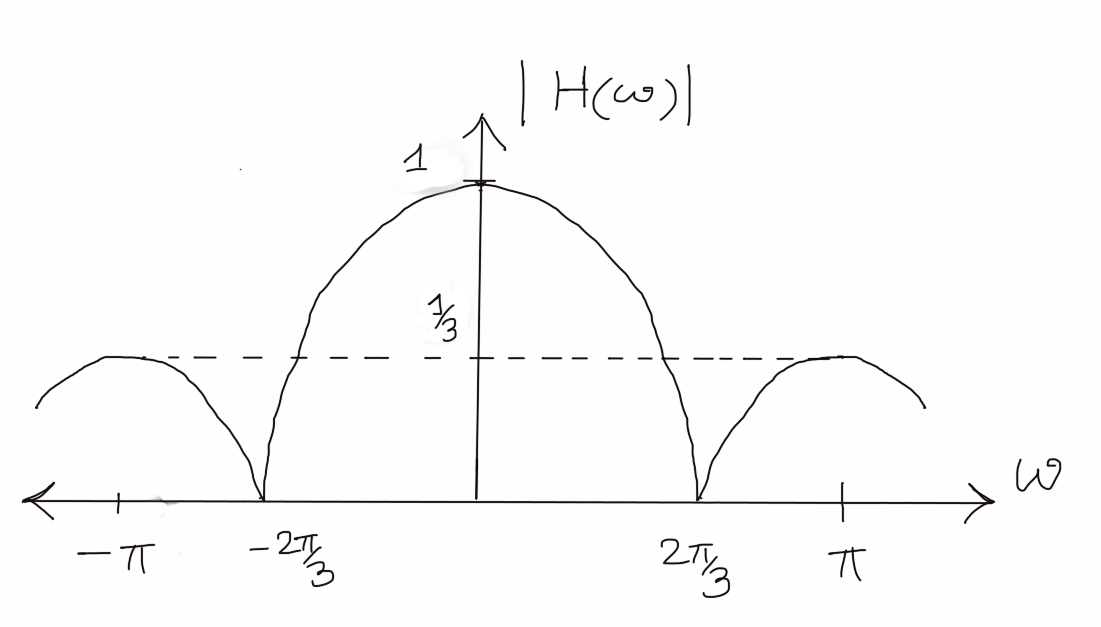
\includegraphics[width = 0.6\linewidth]{img1.png}
            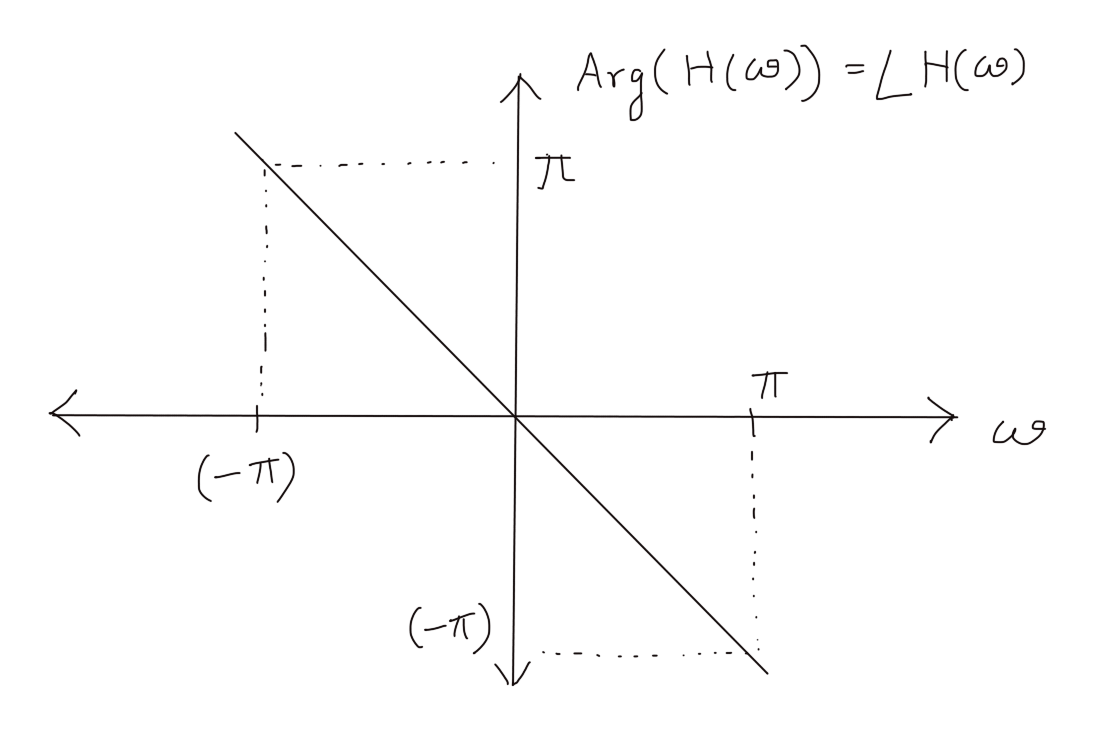
\includegraphics[width = 0.6\linewidth]{img2.png}
        \end{figure}

        Clearly, as the first figure show, the frequency response is $0$ if $\omega = (2\pi/3)$ and is equal to $1$ when $\omega = 0$.
    \end{enumerate}

\end{answer}

% Q4
% DONE
\begin{question}
    Consider the periodic sequence 
    $$
    x_p(n) = \cos\left( \dfrac{2\pi}{10} n\right) \qquad -\infty < n < \infty
    $$
    with frequency $f_0 = (1/10)$ and fundamental period $N = 10$. Determine the $10$-point DFT of the sequence $x(n) = x_p(n)$, $0 \leq n \leq (N-1)$.
\end{question}

\begin{answer}
    Let us denote the $10$-point DFT of $x(n)$ as $X(k)$ for $k = 0, 1, 2, \dots 9$, (as $N = 10$). Thus,

    \begin{align*}
        X(k)
        & = \sum_{n = 0}^{9} x_p(n) e^{-j\frac{2\pi}{10}kn}\\
        & = \sum_{n = 0}^{9} \cos\left( \dfrac{2\pi}{10}n \right) e^{-j\frac{2\pi}{10}kn}\\
        & = \dfrac{1}{2} \left[\sum_{n = 0}^{9} \left(e^{j\frac{2\pi}{10}n} + e^{-j\frac{2\pi}{10}n}\right) e^{-j\frac{2\pi}{10}kn}\right]\\
        & = \dfrac{1}{2} \sum_{n = 0}^{9} e^{-j\frac{2\pi}{10}(k-1)n} + \dfrac{1}{2} \sum_{n = 0}^{9} e^{-j\frac{2\pi}{10}(k+1)n}\\
    \end{align*}

    Now, since $e^{j(2\pi/N)}$ is a $N$-th root of unity, it follows that 

    $$
    \sum_{n = 0}^{N} e^{j(2\pi / N)kn} = \begin{cases}
        N & \text{ if } k = 0, \pm N, \pm 2N, \dots\\
        0 & \text{ otherwise }
    \end{cases}
    $$

    Thus, 

    $$
    X(k) = \begin{cases}
        5 & \text{ if } k = 1, 9\\
        0 \text{ otherwise }
    \end{cases}
    $$

    since $k = 1$ would make the first sum nonzero while $k = 9$ would make the second sum nonzero.
\end{answer}

% Q5
% DONE
\begin{question}
    \begin{enumerate}
        \item[(a)] Determine the Fourier transform $X(\omega)$ of the signal $x(n) = [1, 2, \underset{\uparrow}{3}, 2, 1, 0]$.
        \item[(b)] Compute the $6$-point DFT $V(k)$ of the signal $v(n) = [\underset{\uparrow}{3}, 2, 1, 0, 1, 2]$.
        \item[(c)] Is there any relation between $X(\omega)$ and $V(k)$? Explain.  
    \end{enumerate}
\end{question}

\begin{answer}
    \begin{enumerate}
        \item[(a)] The DTFT $X(\omega)$ of the signal $x(n) = [1, 2, \underset{\uparrow}{3}, 2, 1, 0]$ is 
        
        \begin{align*}
            X(\omega)
            & = \sum_{n = -\infty}^{\infty} x(n) e^{-j\omega n}\\
            & = e^{-2j\omega} + 2 e^{-j\omega} + 3 + 2e^{j\omega} + e^{2j\omega}\\
            & = 3 + 4\cos(\omega) + 2 \cos(2\omega)
        \end{align*}

        \item[(b)] The $6$-point DFT $V(k)$ of the signal $v(n) = [\underset{\uparrow}{3}, 2, 1, 0, 1, 2]$ is given by 
        
        \begin{align*}
            V(k)
            & = \sum_{n = 0}^5 x(n) e^{-j\frac{2\pi}{6}kn}\\
            & = \sum_{n = 0}^5 x(n) e^{-j\frac{\pi}{3}kn}\\
            & = 3 + 2 e^{-j(\pi/3)k} + e^{-j(2\pi/3)k} + e^{-j(4\pi/3)k} + 2e^{-j(5\pi/3)k}\\
            & = 3 + 2 e^{-j(\pi/3)k} + e^{-j(2\pi/3)k} + e^{j(-(4\pi/3)k + 2\pi k)} + 2e^{j(-(5\pi/3)k + 2\pi k)}\\
            & = 3 + 2 e^{-j(\pi/3)k} + e^{-j(2\pi/3)k} + e^{j(2\pi/3)k} + 2e^{j(\pi/3)k}\\
            & = 3 + 4\cos\left(\dfrac{\pi}{3}k\right) + 2\cos\left(\dfrac{2\pi}{3}k\right)\\
        \end{align*}
        
        \item[(c)] It is clear that $V(k) = X(k\pi/3)$ for $k = 0, 1, 2, \dots 5$. The reason for this is that both the signal $x(n)$ or $v(n)$ has the same periodic extension given by 
        $$[\dots, 3, 2, 1, 0, 1, 2, \underset{\uparrow}{3}, 2, 1, 0, 1, 2, 3, 2, 1, 0, 1, 2, \dots]$$ 
        with a fundamental period of length $6$. Hence, the discretized version of $X(\omega)$ at the frequency domain matches the DTFT of the signal $V(k)$.
    \end{enumerate}
\end{answer}

% Q6
\begin{question}
    Prove the identity
    $$
    \sum_{l = -\infty}^\infty \delta(n + lN) = \dfrac{1}{N} \sum_{k = 0}^{N-1} e^{j(2\pi / N)kn}
    $$
\end{question}

\begin{answer}
    We consider the sum $\sum_{k = 0}^{(N-1)} e^{j (2\pi / N)kn}$ first.

    Let, $d = \text{GCD}(n, N)$ where GCD denotes the greatest common divisor function. Note that, if $1 \leq d \leq (N-1)$, then each $e^{j (2\pi / N)kn}$ is a $(N/d)$-th root of unity. To see this, note that 

    $$\left( e^{j (2\pi / N)kn} \right)^{(N/d)} = e^{j(2\pi)kn/d} = 1$$

    since $(n/d)$ is an integer as $d = \text{GCD}(n, N)$. Therefore, the set $\{ e^{j (2\pi / N)kn} : k = 0, 1, \dots (N-1) \}$ is a complete set of $(N/d)$-th roots of unity, counted $d$ times. Since the roots of unity sums up to $0$, we have $\sum_{k = 0}^{(N-1)} e^{j (2\pi / N)kn} = 0$ as long as $1 \leq d \leq (N-1)$. 

    On the other hand, if $d = N$, i.e. $n$ is a multiple of $N$, then $e^{j (2\pi / N)kn} = 1$ for any choice of integer $k$, thus $\sum_{k = 0}^{(N-1)} e^{j (2\pi / N)kn} = N$. 

    Therefore, we have 

    \begin{align*}
        \dfrac{1}{N} \sum_{k = 0}^{(N-1)} e^{j(2\pi/N)kn} 
        & = \begin{cases}
            N/N = 1 & \text{ if } n = lN \text{ for some } l \in \Z\\
            0 & \text{otherwise}
        \end{cases}\\
        & = \sum_{l = -\infty}^{\infty} \delta(n - lN) \\
        & = \sum_{l = -\infty}^{\infty} \delta(n + lN) \qquad \text{substituting } l \text{ in place of } (-l)
    \end{align*}


\end{answer}




% Q7
\begin{question}
    Consider the sequences
    $$
    x_1(n) = [\underset{\uparrow}{0}, 1, 2, 3, 4]
    \qquad 
    x_2(n) = [\underset{\uparrow}{0}, 1, 0, 0, 0]
    \qquad 
    s(n) = [\underset{\uparrow}{1}, 0, 0, 0, 0]
    $$
    and their $5$-point DFTs.
    \begin{enumerate}
        \item[(a)] Determine a sequence $y(n)$ so that $Y(k) = X_1(k)X_2(k)$.
        \item[(b)] Is there a sequence $x_3(n)$ such that $S(k) = X_1(k)X_3(k)$? 
    \end{enumerate}
\end{question}

\begin{answer}
    We first compute the $5$-point DFT of the given sequences.

    \begin{align*}
        X_1(k) 
        & = \sum_{n = 0}^4 x_1(n) e^{-j(2\pi/5)k n}\\
        & = e^{-j(2\pi/5)k} + 2 e^{-j(4\pi/5)k} + 3e^{-j(6\pi/5)k} + 4e^{-j(8\pi/5)k}\\
        & = e^{-j(2\pi/5)k} + 2 e^{-j(4\pi/5)k} + 3e^{j(4\pi/5)k} + 4e^{j(2\pi/5)k}\\
        & = \left[ 5 \cos\left( \dfrac{2\pi}{5}k \right) + 5 \cos\left( \dfrac{4\pi}{5}k \right)\right] + \left[ 3 \sin\left( \dfrac{2\pi}{5}k \right) + \sin\left( \dfrac{4\pi}{5}k \right) \right] j
    \end{align*}

    and 

    $$
    X_2(k) = \sum_{n = 0}^4 x_2(n) e^{-j(2\pi/5)k n} = e^{-j(2\pi/5)k} = \cos\left( \dfrac{2\pi}{5}k \right) - j \sin\left( \dfrac{2\pi}{5}k \right)
    $$

    and 

    $$
    S(k) = \sum_{n = 0}^4 s(n) e^{-j(2\pi/5)k n} = 1
    $$

    for $k = 0, 1, 2, 3, 4$.

    \begin{enumerate}
        \item[(a)] We want $y(n)$ so that $Y(k) = X_1(k)X_2(k)$. Note that,
        
        \begin{align*}
            X_1(k) X_2(k)
            & = e^{-j(2\pi/5)k} \left[ e^{-j(2\pi/5)k} + 2 e^{-j(4\pi/5)k} + 3e^{j(4\pi/5)k} + 4e^{j(2\pi/5)k} \right]\\
            & = e^{-j(4\pi/5)k} + 2e^{-j(6\pi/5)k} + 3 e^{j(2\pi/5)k} + 4 \\
            & = 4 + e^{-j(4\pi/5)k} + 2e^{-j(6\pi/5)k} + 3 e^{-j(8\pi/5)k}\\
            & = \text{DFT}\left( [\underset{\uparrow}{4}, 0, 1, 2, 3] \right)
        \end{align*}

        Therefore, the sequence $y(n)$ so that $Y(k) = X_1(k)X_2(k)$, is given by $[\underset{\uparrow}{4}, 0, 1, 2, 3]$.

        \item[(b)] Let, $x_3(n) = [a, b, c, d, e]$. Since by hypothesis, $S(k) = X_1(k)X_3(k)$ and discrete circular convolution is elementwise product in discrete frequency domain, it then follows that $s(n)$ is a circular convolution of $x_1(n)$ and $x_3(n)$. Thus,
        
        $$
        s(m) = \sum_{n = 0}^{4} x_1(n) x_2\left( (m - n) \right)_5, \qquad m = 0, 1, 2, 3, 4
        $$

        Therefore, we have the system of equations

        \begin{align*}
            1 = s(0) & = (e + 2d + 3c + 4b)\\
            0 = s(1) & = (a + 2e + 3d + 4c)\\
            0 = s(2) & = (b + 2a + 3e + 4d)\\
            0 = s(3) & = (c + 2b + 3a + 4e)\\
            0 = s(4) & = (d + 2c + 3b + 4a)\\             
        \end{align*}

        i.e. 

        $$
        \begin{bmatrix}
            0 & 4 & 3 & 2 & 1\\
            1 & 0 & 4 & 3 & 2\\
            2 & 1 & 0 & 4 & 3\\
            3 & 2 & 1 & 0 & 4\\
            4 & 3 & 2 & 1 & 0\\
        \end{bmatrix} \begin{bmatrix}
            a \\ b\\ c\\ d\\ e
        \end{bmatrix} = \begin{bmatrix}
            1 \\ 0 \\ 0\\ 0 \\ 0
        \end{bmatrix}
        $$

        Solving this, we have the solution as 

        $$
        x_3(n) = \left[ -\dfrac{9}{50}, \dfrac{11}{50}, \dfrac{1}{50}, \dfrac{1}{50}, \dfrac{1}{50} \right]
        $$

        which is the desired sequence $x_3(n)$ such that $S(k) = X_1(k)X_3(k)$ for $k = 0, 1, \dots 4$.
    \end{enumerate}

\end{answer}



% Q8
\begin{question}
    A linear time invariant system with frequency response $H(\omega)$ is excited with the periodic input 
    $$
    x(n) = \sum_{k = -\infty}^\infty \delta(n - kN)
    $$
    Suppose that we compute the $N$-point DFT $Y(k)$ of the samples $y(n)$, $0 \leq n \leq (N-1)$ of the output sequence. How is $Y(k)$ related to $H(\omega)$?
\end{question}

\begin{answer}
    Let, $h(n)$ be the impulse response function of the system. Then, we know that the output of the LTI system $y(n) = h(n) \ast x(n)$, where $x(n)$ is the input signal. Computing the $N$-point DFT of $y(n)$, we obtain 

    \begin{align*}
        Y(k)
        & = \sum_{n = 0}^{(N-1)} y(n) e^{-j(2\pi / N)kn}\\
        & = \sum_{n = 0}^{(N-1)} \left[\sum_{r = -\infty}^{\infty} h(r) x(n-r)\right] e^{-j(2\pi / N)kn}\\
        & = \sum_{n = 0}^{(N-1)} \left[\sum_{r = -\infty}^{\infty} h(r) \sum_{l = -\infty}^\infty \delta(n - r - lN)\right] e^{-j(2\pi / N)kn}
    \end{align*}
    Now, interchanging the sums yield,

    \begin{align*}
        Y(k) & = \sum_{r = -\infty}^{\infty} h(r) \sum_{n = 0}^{(N-1)} \sum_{l = -\infty}^\infty \delta(n - r - lN) e^{-j(2\pi / N)k(n - r)} e^{-j(2\pi / N)kr}\\
        & = \sum_{r = -\infty}^{\infty} h(r) \sum_{n = 0}^{(N-1)} \sum_{l = -\infty}^\infty \delta(n - r - lN) e^{-j(2\pi / N)k(n - r - lN)} e^{-j(2\pi / N)kr}\\
        & \qquad \qquad \text{since, } e^{j(2\pi/N) lN} = e^{j(2\pi)l} = 1, \quad \forall l \in \Z\\
        & = \sum_{r = -\infty}^{\infty} h(r) \sum_{l = -\infty}^\infty \sum_{m = lN}^{lN + (N-1)} \delta(m) e^{-j(2\pi/N)km} e^{-j(2\pi/N)kr}\\
        & \qquad \qquad \text{assuming, } m = (n - r - lN)\\
        & = \sum_{r = -\infty}^{\infty} h(r)e^{-j(2\pi/N)kr} \qquad \text{since, } \delta(m) = 0 \text{ iff } m = 0\\
        & = H\left( \dfrac{2\pi}{N}k \right)
    \end{align*}
    
    where $H(\omega)$ is the DTFT of the impulse response (i.e. the frequency response) of the given LTI system.
\end{answer}


% Q9
\begin{question}
    Show that each of the numbers $e^{j(2\pi / N)k}$ for $0 \leq k \leq (N-1)$ corresponds to an $N$-th root of units. Plot these numbers as phasors in the complex plane and illustrate, by means of this figure, the orthogonality property
    $$
    \sum_{n = 0}^{(N-1)} e^{j(2\pi / N)kn} e^{-j(2\pi / N)ln} = \begin{cases}
        N & \text{ if } k = l\\
        0 & \text{ if } k \neq l\\
    \end{cases}
    $$
\end{question}

\begin{answer}
    Clearly note that, 

    $$
    \left( e^{j(2\pi / N)k}\right)^N = e^{j(2\pi / N)Nk} = e^{j(2\pi k)} = (e^{j(2\pi)})^k = 1
    $$

    since $k$ is an integer, and $e^{j(2\pi)} = 1$. Thus, these numbers corresponds to an $N$-th root of unity. The following figure depicts the position of these numbers on the complex plane. For ease of illustration, we use $N = 12$.

    \begin{figure}[H]
        \centering
        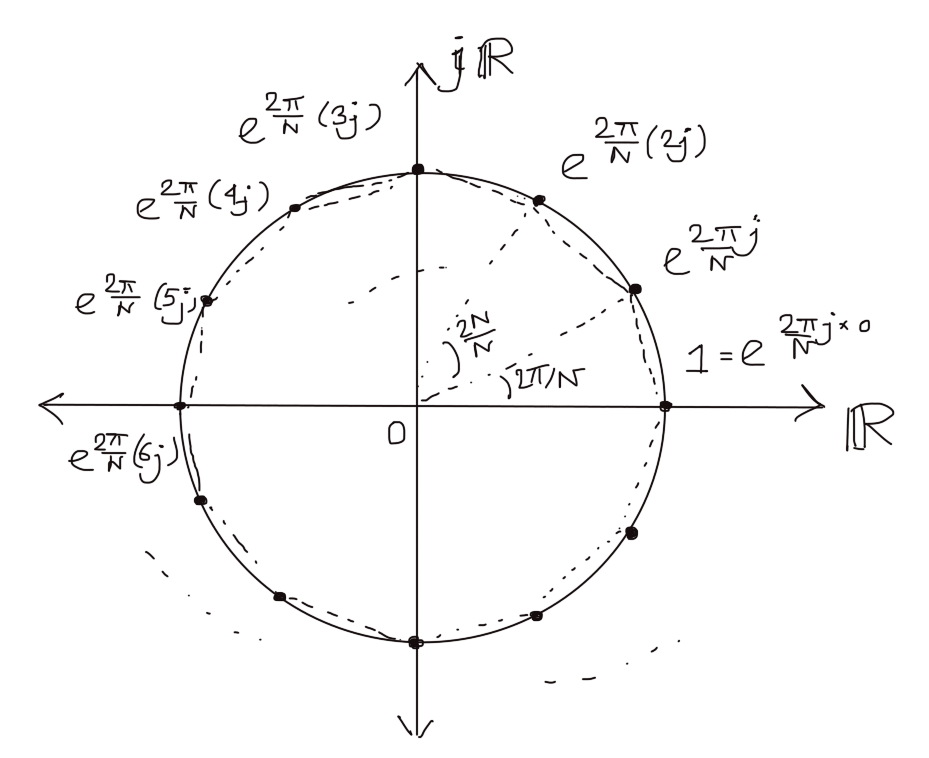
\includegraphics[width = 0.7\linewidth]{img3.png}
    \end{figure}


    Note that, $\sum_{n = 0}^{(N-1)} e^{j(2\pi / N)kn} e^{-j(2\pi / N)ln} = \sum_{n = 0}^{(N-1)} e^{j(2\pi / N)(k-l)n}$. If $k = l$ (i.e. $(k-l) = 0$), then clearly each of these terms is equal to $1$, and there are $N$ such terms, summing up to $N$.

    So, let us assume $k \neq l$ and without loss of generality assume $k > l$. Denoting $(k - l) = r$, we see that $1 \leq r \leq (N-1)$. Since $r \neq 0$, we define $d = \text{GCD}(N, r)$, where $\text{GCD}$ is the greatest common divisor function. Clearly, each of the terms $e^{j(2\pi / N)(k-l)n} = e^{j(2\pi / N)rn}$ is now a $(N/d)$-th root of unity, and taking all of these summands together will comprise of $d$ such full sets of $(N/d)$-th roots of unity. However, as shown in the figure, the roots of unity lies on the unit circle forming a regular polygon of unit circumradius, centered at the origin. Since the polygon is regular, by symmetry it follows that the center of mass of the polygon must be at the origin. But we also know that the center of mass would be at the position given by the arithmetic mean of the vertex coordinates. In other words, this imply 

    $$
    \dfrac{1}{N} \sum_{n = 0}^{(N-1)} e^{j(2\pi / N)rn} = 0\qquad \forall 1 \leq r \leq (N-1)
    $$

    i.e.

    for $k > l$, 

    $$
    \sum_{n = 0}^{(N-1)} e^{j(2\pi / N)(k-l)n} = 0
    $$

    The case $k < l$ follows from symmetry. Thus, combining everything, we obtain the orthogonality property,

    $$
    \sum_{n = 0}^{(N-1)} e^{j(2\pi / N)kn} e^{-j(2\pi / N)ln} = \begin{cases}
        N & \text{ if } k = l\\
        0 & \text{ if } k \neq l\\
    \end{cases}
    $$
    
\end{answer}





% Q10
\begin{question}
    Derive the signal flow graph for the $N = 16$ point, radix $4$ decimation in time FFT algorithm in which the input sequence is in normal order and the computations are done in place.
\end{question}

\begin{answer}
    Note that, radix-$4$ decimation in time FFT algorithm uses a divide and conquer approach to compute $4$ DFT of subsequences of the original input sequence, and then uses some overhead calculation to combine all $4$ DFT's. Now to compute $16$-point DFT, we consider

    \begin{align*}
        X[k]
        & = \sum_{n = 0}^{15} x(n) e^{-j(2\pi/16)kn}\\
        & = \sum_{r = 0}^{3} \sum_{l = 0}^{3} x(4l + r) e^{-j(2\pi/16)k(4l + r)}\\
        & = \sum_{r = 0}^{3} e^{-j(2\pi/16)rk} \sum_{l = 0}^{3} x(4l + r) e^{-j(2\pi/4)kl}\\
        & = \text{DFT}_{N/4}[x(4n)] + W_N^k \text{DFT}_{N/4}[x(4n+1)] + W_N^{2k}\text{DFT}_{N/4}[x(4n+2)] + W_N^{3k}\text{DFT}_{N/4}[x(4n+3)]
    \end{align*}

    where $\text{DFT}_{N/4}$ denotes the $N/4 = 4$-point DFT and $W_N$ denotes a proper $16$-th root of unity. Now, if we denote these $4$-point DFTs as,

    \begin{align*}
        \text{DFT}\{ x(0), x(4), x(8), x(12) \} & = G_1(l), l = 0, 1, 2, 3\\
        \text{DFT}\{ x(1), x(5), x(9), x(13) \} & = G_2(l), l = 0, 1, 2, 3\\
        \text{DFT}\{ x(2), x(6), x(10), x(14) \} & = G_3(l), l = 0, 1, 2, 3\\
        \text{DFT}\{ x(3), x(7), x(11), x(15) \} & = G_4(l), l = 0, 1, 2, 3\\
    \end{align*}

    Then, since each $N/4$-point DFT's are periodic in nature with period equal to $N / 4 = 4$ samples, we have

    $$
    X[k] = G_1(k) + W_N^{k} G_2(k) + W_N^{2k} G_3(k) + W_N^{3k} G_4(k), \qquad k = 0, 1, \dots 15
    $$

    i.e.,

    $$
    X[k] = \begin{cases}
        G_1(0) + G_2(0) + G_3(0) + G_4(0), & k = 0\\
        G_1(1) + W_N G_2(1) + W_N^2 G_3(1) + W_N^{3} G_4(1), & k = 1\\
        G_1(2) + W_N^2 G_2(2) + j G_3(2) + j W_N^{2} G_4(2), & k = 2\\
        G_1(3) + W_N^3 G_2(3) + j W_N^{2} G_3(3) - W_N G_4(3), & k = 3\\
        G_1(0) + j G_2(0) - G_3(0) - j G_4(0), & k = 4\\
        G_1(1) + j W_N G_2(1) - W_N^{2} G_3(1) - j W_N^{3} G_4(1), & k = 5\\
        G_1(2) + j W_N^2 G_2(2) - j G_3(2) + W_N^{2} G_4(2), & k = 6\\
        G_1(3) + j W_N^3 G_2(3) - j W_N^{2} G_3(3) +  j W_N G_4(3), & k = 7\\
        G_1(0) - G_2(0) + G_3(0) - G_4(0), & k = 8\\
        G_1(1) - W_N G_2(1) + W_N^2 G_3(1) - W_N^{3} G_4(1), & k = 9\\
        G_1(2) - W_N^2 G_2(2) + j G_3(2) - j W_N^{2} G_4(2), & k = 10\\
        G_1(3) - W_N^3 G_2(3) + j W_N^{2} G_3(3) +  W_N G_4(3), & k = 11\\
        G_1(0) - j G_2(0) - G_3(0) + j G_4(0), & k = 12\\
        G_1(1) - j W_N G_2(1) - W_N^{2} G_3(1) + j W_N^{3} G_4(1), & k = 13\\
        G_1(2) - j W_N^2 G_2(2) - j G_3(2) - W_N^{2} G_4(2), & k = 14\\
        G_1(3) - j W_N^3 G_2(3) - j W_N^{2} G_3(3) - j W_N G_4(3), & k = 15\\
    \end{cases} 
    $$

    The following diagram shows the signal flow graph of this radix-4 16-point decimation-in-time DFT algorithm. The coefficients has been suppressed due to clarity of the figure.

    \begin{figure}[H]
        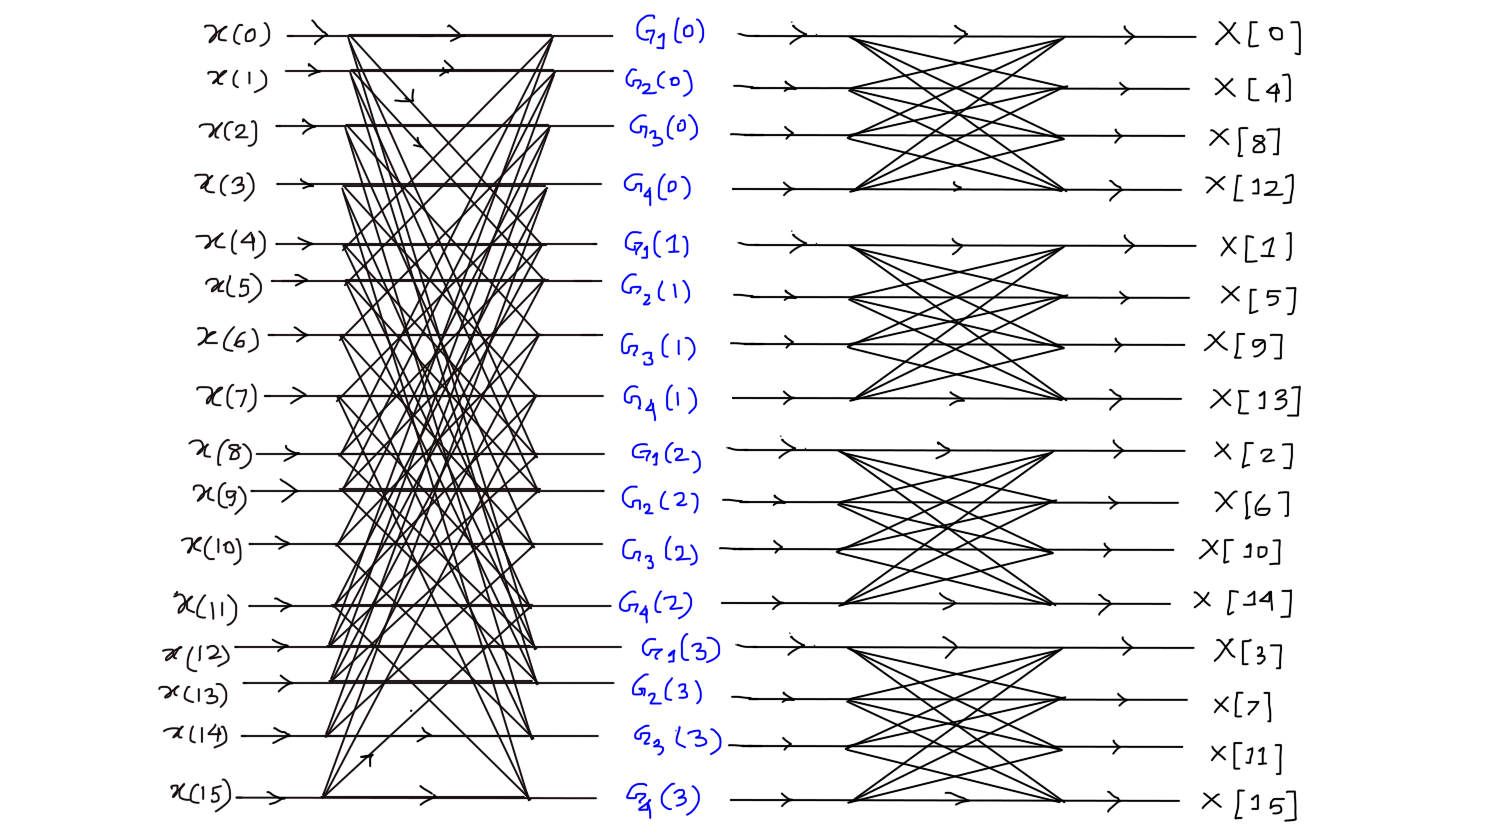
\includegraphics[width = \linewidth]{fft-radix4.png}
    \end{figure}

\end{answer}



% Q11
\begin{question}
    Compute the $16$-point DFT of the sequence $x(n) = \cos((\pi/2)n)$ for $0 \leq n \leq 15$ using the radix-4 decimation in time algorithm.
\end{question}

\begin{answer}
    Since the given input signal is $x(n) = \cos((\pi/2)n)$ for $0 \leq n \leq 15$, we write the input sequence by computing its elements as 

    $$
    x(n) = [\underset{\uparrow}{1}, 0, -1, 0, 1, 0, -1, 0, 1, 0, -1, 0, 1, 0, -1, 0]
    $$

    We need to compute the $16$-point DFT using radix-4 decimation in time algorithm, thus, we start by considering $4$-point DFT of certain subsequences of the input sequence.

    First, we start by computing the $4$-point DFT of the sequence $[x(0), x(4), x(8), x(12)] = [1, 1, 1, 1]$. Denoting this by $G_1$, we have 

    $$
    G_1(k) = 1^k + i^k + (-1)^k + (-i)^k = \begin{cases}
        4 & \text{ if } k = 0\\
        0 & \text{ otherwise}
    \end{cases}, \qquad k = 0, 1, 2, 3
    $$

    Next, we have the $4$-point DFT $H_1$ of $[x(2), x(6), x(10), x(14)] = [-1, -1, -1, -1]$, which similar to above turns out to be, 

    $$
    H_1(k) = \begin{cases}
        (-4) & \text{ if } k = 0\\
        0 & \text{ otherwise} 
    \end{cases}, \qquad k = 0, 1, 2, 3
    $$

    Note that, the $4$-point DFT of the sequences $[x(1), x(5), x(9), x(13)]$ and $[x(3), x(7), x(11), x(15)]$ will be equal to $0$, since all values of these subsequences are $0$'s. We denote these $4$-point DFT's as $G_2$ and $H_2$ respectively. 

    In the next step of the radix-4 decimation-in-time algorithm, these DFT's will be taken together to output the final $16$ point DFT by the overhead operation shown in the answer to the previous question. Since, $G_2$ and $H_2$'s equal to $0$, it follows that, 

    \begin{align*}
        X[k]
        & = G_1(k) + w^k G_2(k) + w^{2k} H_1(k) + w^{3k} H_2(k)\\
        & = G_1(k) + w^{2k} H_1(k)\\
    \end{align*}

    where $w$ is a $16$-th root of unity, namely $w = e^{(2\pi/16)j}$. Also, since $G_1(k)$ and $H_1(k)$ are nonzero if and only if $k$ is multiple of $4$ (due to the periodicity of $4$-point DFT), we have 

    $$
    X[k] = \begin{cases}
        G_1(0) + w^0 H_1(0) = 4 + (-4) = 0, & k = 0\\
        G_1(4) + w^8 H_1(4) = 4 - (-4) = 8, & k = 4\\
        G_1(8) + w^{16} H_1(8) = 4 + (-4) = 0, & k = 8\\
        G_1(12) + w^{24} H_1(12) = 4 - (-4) = 8, & k = 12\\
        G_1(k) + w^k H_1(k) = 0 + 0 = 0, & \text{otherwise}\\
    \end{cases}
    $$


    Thus, it follows that the final $16$-point DFT of the given sequence is given by

    $$
    X[k] = \begin{cases}
        8 & \text{ if } k = 4, 12\\
        0 & \text{ otherwise }
    \end{cases}
    $$
    
\end{answer}



% DONE
% Q12
\begin{question}
    Let $X(k)$ be the $N$ point DFT of the sequence $x(n)$ for $0 \leq n \leq (N-1)$. We define $2N$-point sequence $y(n)$ as
    $$
    y(n) = \begin{cases}
        x(n/2) & n \text{ even}\\
        0 & n \text{ odd}
    \end{cases}
    $$

    Express the $2N$-point DFT of $y(n)$ in terms of $X(k)$.
\end{question}

\begin{answer}
    The $2N$-point DFT of $y(n)$ is given by,
    \begin{align*}
        Y_{2N}(k)
        & = \sum_{n = 0}^{(2N - 1)} y(n) e^{-j(2\pi/2N)kn}\\
        & = \sum_{\substack{n = 0\\n \text{is even}}}^{(2N - 1)} x(n/2) e^{-j(2\pi/2N)kn}\\
        & = \sum_{m = 0}^{(N-1)} x(m)e^{-j(2\pi/2N)(2m)k} \qquad \text{where, } m = (n/2)\\
        & = \sum_{m = 0}^{(N-1)} x(m)e^{-j(2\pi/N)mk}\\
        & = X(k)
    \end{align*}

    Thus, the $2N$-point DFT of $y(n)$ is a repeated version of $X(k)$, in other words, for $0 \leq k \leq (2N-1)$,

    $$
    Y_{2N}(k) = \begin{cases}
        X(k) & \text{if } 0 \leq k \leq (N-1)\\
        X(k-N) & \text{if } N \leq k \leq (2N-1)\\
    \end{cases}
    $$
\end{answer}



\end{document}
